\documentclass[tikz, border=10pt]{standalone}

% preamble
\usepackage{tikz}
\usetikzlibrary{mindmap, shadows}
\usepackage[hidelinks, pdfencoding=auto]{hyperref}

% define styles
\tikzset{
    every annotation/.style = {draw=cyan!50!black, line width=1.5pt, fill=green!10, font=\Large},
    every node/.style = {concept, circular drop shadow},
    root/.style = {concept color=black!40, font=\large\bfseries, text width=10em},
    level 1 concept/.append style = {font=\Large\bfseries, sibling angle=50, text width=7.7em, level distance=15em, inner sep=0pt},
    level 2 concept/.append style = {font=\bfseries, level distance=9em}
}

% create information box, \info requires 4 arguments
% the first arg: text width (default 16.3 em)
% the second arg: position in which box is placed
% the third arg: node options
% the last arg: items list
\newcommand*{\info}[4][16.3]{
    \node[annotation, #3, scale=0.65, text width=#1 em,inner sep=2mm] at (#2){
        \list{$\bullet$}{
            \topsep=0pt\itemsep=0pt\parsep=0pt\parskip=0pt
            \labelwidth=8pt\leftmargin=8pt\itemindent=0pt
            \labelsep=2pt
        }
        #4
        \endlist
    };
}

\begin{document}
    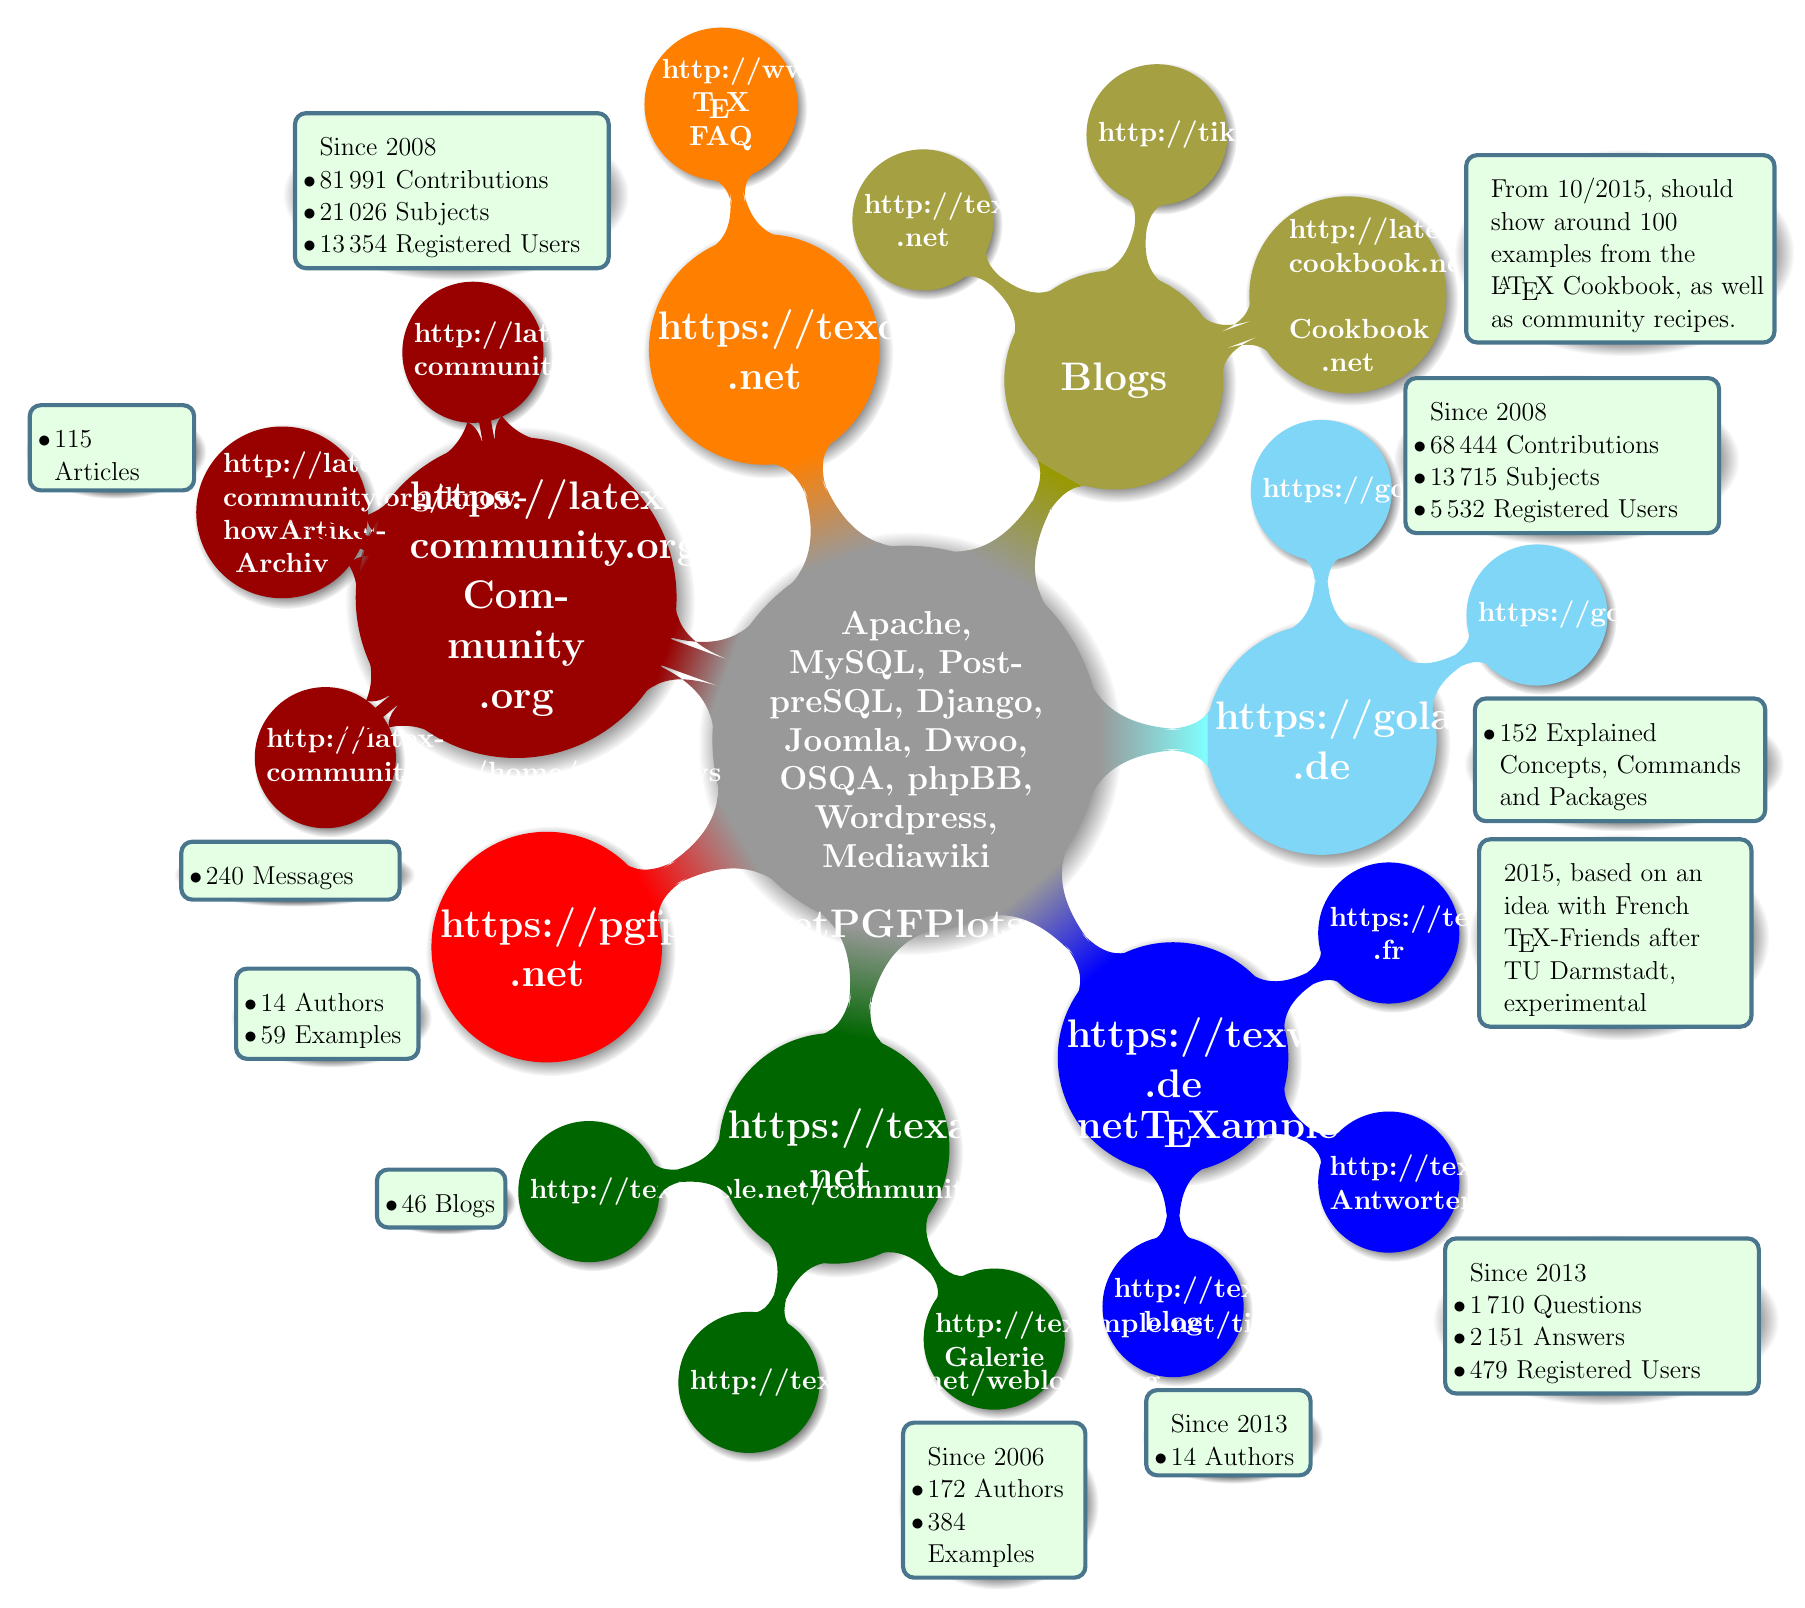
\begin{tikzpicture}
        \path[mindmap, concept color=black!40, text=white]              
            node[root] {Apache, MySQL, PostpreSQL, Django, Joomla, Dwoo, OSQA, phpBB, Wordpress, Mediawiki}
            [clockwise from=0]
            child[concept color=cyan!50]{
                node{\href{https://golatex.de}{go\LaTeX\\.de}}
                [clockwise from=90]
                child { node[concept] (goForum) {\href{https://golatex.de/index.html}{Forums}}}
                child { node[concept] (goWiki){\href{https://golatex.de/wiki/Hauptseite}{Wiki}}}
            }
            child[concept color=blue]{
                node[concept] {\href{https://texwelt.de/}{\TeX welt\\.de}}
                [clockwise from=30]
                child { node[concept] (TeXnique) {\href{https://texnique.fr}{\TeX nique\\.fr}}}
                child { node[concept] (TeXweltQA) {\href{http://texwelt.de/wissen/}{Fragen~\& Antworten}}}
                child { node[concept] (TeXweltBlog) {\href{http://texwelt.de/blog/}{User blog}}}
            }
            child[concept color=green!40!black]{
                node[concept] {\href{https://texample.net}{\TeX ample\\.net}}
                [clockwise from=310]
                child { node[concept] (TikZGalerie) {\href{http://texample.net/tikz/examples/}{TikZ-Galerie}}}
                child { node[concept] (TeXampleBlog) {\href{http://texample.net/weblog/}{Blog}}}
                child { node[concept] (Planet) {\href{http://texample.net/community/}{Planet}}}
            }
            child[concept color=red]{
                node[concept] (PGFPlots) {\href{https://pgfplots.net}{PGFPlots\\.net}}
                [clockwise from=270]
            }
            child[concept color=red!60!black] {
                node[concept] {\href{https://latex-community.org}{\LaTeX{} Community\\.org}}
                [counterclockwise from=100]
                child { node[concept] (LaTeXForum) {\href{http://latex-community.org/forum/}{Forum}}}
                child { node[concept] (LaTeXArtikel) {\href{http://latex-community.org/know-how}{Artikel-Archiv}}}
                child { node[concept] (LaTeXNews) {\href{http://latex-community.org/home/news}{News}}}
            }
            child[concept color=orange]{
                node[concept] (TeXdoc) {\href{https://texdoc.net}{\TeX doc\\.net}}
                [clockwise from=100]
                child { node[concept] {\href{http://www.tex.ac.uk}{UK \TeX \\FAQ}}}
            }
            child[concept color=yellow!60!black]{
                node[concept] {Blogs}
                [clockwise from=140]
                child { node[concept] {\href{http://texblog.net/}{\TeX blog\\.net}}}
                child { node[concept] {\href{http://tikz.de/}{TikZ.de}}}
                child { node[concept] (Cookbook) {\href{http://latex-cookbook.net/}{\LaTeX-\\Cookbook\\.net}}}
            };
        \info {goForum.north east}{above,anchor=west,shift={(1em, -0.5em)}}{%
            \item[] Since 2008
            \item 68\,444 Contributions
            \item 13\,715 Subjects
            \item 5\,532 Registered Users
        }
        \info {LaTeXForum.north west}{above,anchor=south, shift={(1em, 1em)}}{%
            \item[] Since 2008
            \item 81\,991 Contributions
            \item 21\,026 Subjects
            \item 13\,354 Registered Users
        }
        \info [8]{LaTeXArtikel.north west}{below,anchor=north east,shift={(-0.75em, 2em)}}{%
            \item 115 Articles
        }
        \info [11]{LaTeXNews.south west}{below,anchor=north, shift={(0.5em, -1em)}}{%
            \item 240 Messages
        }   
        \info [9]{TikZGalerie.south}{below,anchor=north, shift={(0, -0.25em)}}{%
            \item[] Since 2006
            \item 172 Authors
            \item 384 Examples
        }
        \info [15]{goWiki.south}{below,anchor=north,shift={(3em, -0.25em)}}{%
            \item 152 Explained Concepts, Commands and Packages
        }
        \info {TeXweltQA.south east}{above,anchor=north west}{%
            \item[] Since 2013
            \item 1\,710 Questions
            \item 2\,151 Answers
            \item 479 Registered Users
        }
        \info [8]{TeXweltBlog.south}{below,anchor=north,shift={(2em, -0.25em)}}{%
            \item[] Since 2013
            \item 14 Authors
        }
        \info[9]{PGFPlots.west}{anchor=north east,shift={(-.25em, -0.5em)}}{%
            \item 14 Authors
            \item 59 Examples
        }
        \info [6]{Planet.west}{anchor=east, shift={(-0.25em, -0.25em)}}{%
            \item 46 Blogs
        }
        \info [14]{TeXnique.east}{anchor=west,xshift = 0.5em}{%
            \item[] 2015, based on an idea with French
              \TeX-Friends after TU Darmstadt, experimental
        }
        \info [16]{Cookbook.east}{anchor=south west, shift={(0.5em, -2em)}}{%
            \item[] From 10/2015, should show around 100 examples from the \LaTeX \ Cookbook, as well as community recipes.
        }
    \end{tikzpicture}
\end{document}